\documentclass{article}
\usepackage[a3paper,margin=0.5cm,landscape]{geometry}
\usepackage[utf8]{inputenc}
\usepackage{graphicx,subfigure,tikz,pgfplots,hyperref}

\usepackage[dvipsnames]{xcolor}

\definecolor{primary}{RGB}{101,195,186} % Green
\definecolor{secondary}{RGB}{203,204,198} % Grey
\definecolor{thirdly}{RGB}{248,137,141} % Peach

\pgfplotsset{compat=newest} 
\pgfdeclarelayer{background}    
\pgfsetlayers{background,main}  

\usepackage{fancyhdr}
\usepackage{lastpage}

\fancyhf{} % empty header and footer
\renewcommand{\headrulewidth}{0pt} % ho header line
\renewcommand{\footrulewidth}{0pt}% not footer line
\fancyfoot[C]{Page \thepage\ of \pageref{LastPage}}

\usepackage[font=Large]{caption}

\usetikzlibrary{tikzmark,calc,spy}
\usetikzlibrary{arrows,shapes,positioning,shadows,trees,mindmap}

\begin{document}

\section*{Histogram Analysis}
	\vspace*{-0.4cm}\rule{10cm}{0.1mm}
	
	\Large{This algorithm analyses the brain as a whole volume. The input is a MEMPRAGE image, along with the segmentation files from Freesurfer for white and cortical gray matter segmentation. An example of a coronal slice, cortical gray matter masked and white matter mask used to compute the histograms can be viewed here.} 
	
	\begin{figure}[!h]
        \centering
            \begin{minipage}{0.17\linewidth}
                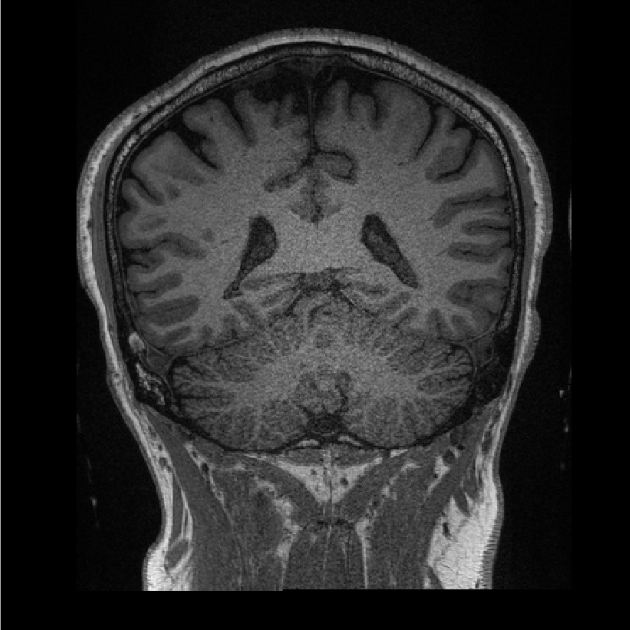
\includegraphics[width=\textwidth]{figures/full_head.png}
            \end{minipage}
            \begin{minipage}{0.17\linewidth}
                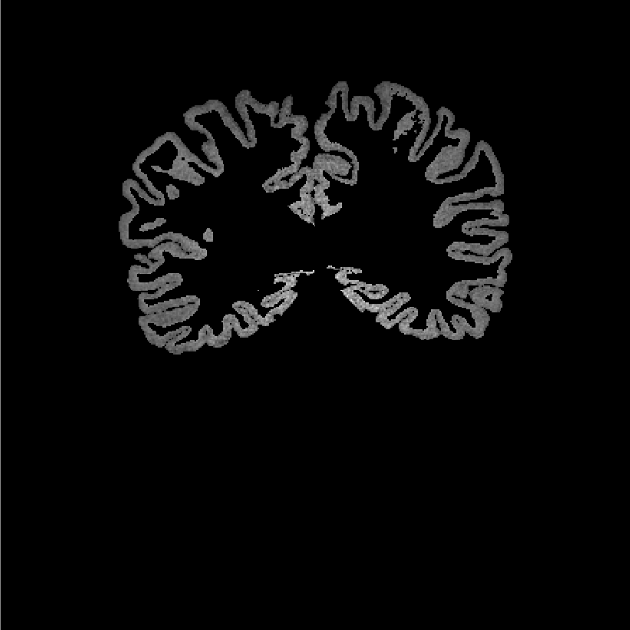
\includegraphics[width=\textwidth]{figures/gray_matter.png}
            \end{minipage}
            \begin{minipage}{0.17\linewidth}
                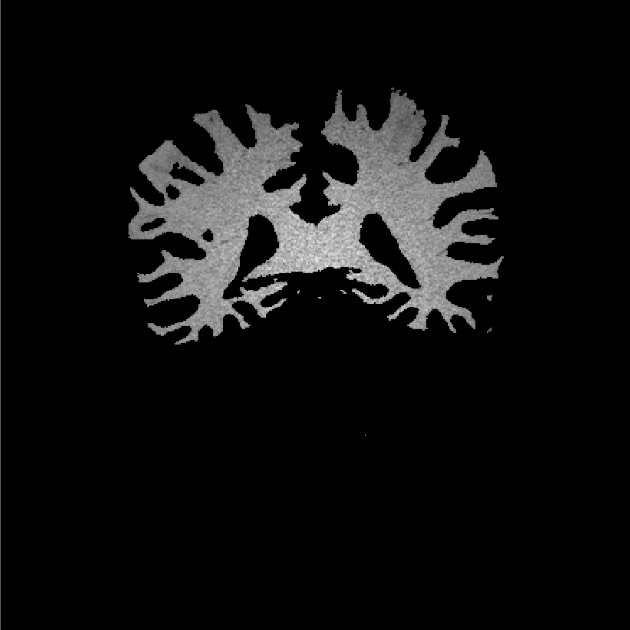
\includegraphics[width=\textwidth]{figures/white_matter.png}
            \end{minipage}
            
            \begin{minipage}{0.17\linewidth}
                \centering MEMPRAGE - coronal slice
            \end{minipage}
            \begin{minipage}{0.17\linewidth}
                \centering cortical gray matter mask
            \end{minipage}
            \begin{minipage}{0.17\linewidth}
                \centering white matter mask
            \end{minipage}
            \vspace{-1cm}
    \end{figure}

\subsection*{MRI Raw Analysis}
	\vspace*{-0.5cm}\rule{5cm}{0.1mm}
	
	\Large{Six MR images using the MEMPRAGE sequence were acquired from a Siemens 3T TrioTrim MR scanner, with a 0.5mm isotropic voxel size (TR=2530ms, TE=2.45, BW=548Hz/px, 480x480 matrix, 3D acquisition). By using the white and cortical gray matter masks, a histogram was computed for each acquisition.} 
	
    \begin{figure}[!h]
        \centering
        \begin{minipage}{0.17\linewidth}
             \begin{tikzpicture}[scale=1]
                \begin{axis}[
                            yticklabels={,,},
                            xtick=data,
                            xticklabels={$0$,,,,,,,,,$0.5$,,,,,,,,,$1$},
                            legend style={at={(0.78,0.98)},
	                        anchor=north,legend columns=-1},
                            ymajorgrids={true},
                            xmajorgrids={true},
                            %grid=major, 
                            grid style={dashed,gray!10},
                            legend style={color=gray,fill=none}
                            ] 
                            \addplot[smooth, color=primary!80!black, mark=star, fill opacity=0.5, opacity=0.5]
                            table[x=index,y=gm_mean,col sep=comma]{matrix/final_matrix_tp5tomean1to6.csv};
                            \addlegendentry{\footnotesize{\color{gray}GM}}
                            \addplot[smooth, color=secondary!80!black, mark=x, fill opacity=0.5, opacity=0.5]
                            table[x=index,y=wm_gm_mean,col sep=comma]{matrix/final_matrix_tp5tomean1to6.csv};
                            \addlegendentry{\footnotesize{\color{gray}WM}};
                \end{axis}
            \end{tikzpicture}\vspace*{-0.5cm}\hspace{0.4cm}
        \end{minipage}
        \begin{minipage}{0.17\linewidth}
             \begin{tikzpicture}[scale=1]
                \begin{axis}[
                            yticklabels={,,},
                            xtick=data,
                            xticklabels={$0$,,,,,,,,,$0.5$,,,,,,,,,$1$},
                            legend style={at={(0.78,0.98)},
	                        anchor=north,legend columns=-1},
                            ymajorgrids={true},
                            xmajorgrids={true},
                            %grid=major, 
                            grid style={dashed,gray!10},
                            legend style={color=gray,fill=none}
                            ] 
                            \addplot[smooth, color=primary!80!black, mark=star, fill opacity=0.5, opacity=0.5]
                            table[x=index,y=gm_mean,col sep=comma]{matrix/final_matrix_tp2tomean1to6.csv};
                            \addlegendentry{\footnotesize{\color{gray}GM}}
                            \addplot[smooth, color=secondary!80!black, mark=x, fill opacity=0.5, opacity=0.5]
                            table[x=index,y=wm_gm_mean,col sep=comma]{matrix/final_matrix_tp2tomean1to6.csv};
                            \addlegendentry{\footnotesize{\color{gray}WM}};
                \end{axis}
            \end{tikzpicture}\vspace*{-0.5cm}\hspace{0.4cm}
        \end{minipage}
        \begin{minipage}{0.17\linewidth}
             \begin{tikzpicture}[scale=1]
                \begin{axis}[
                            yticklabels={,,},
                            xtick=data,
                            xticklabels={$0$,,,,,,,,,$0.5$,,,,,,,,,$1$},
                            legend style={at={(0.78,0.98)},
	                        anchor=north,legend columns=-1},
                            ymajorgrids={true},
                            xmajorgrids={true},
                            %grid=major, 
                            grid style={dashed,gray!10},
                            legend style={color=gray,fill=none}
                            ] 
                            \addplot[smooth, color=primary!80!black, mark=star, fill opacity=0.5, opacity=0.5]
                            table[x=index,y=gm_mean,col sep=comma]{matrix/final_matrix_tp4tomean1to6.csv};
                            \addlegendentry{\footnotesize{\color{gray}GM}}
                            \addplot[smooth, color=secondary!80!black, mark=x, fill opacity=0.5, opacity=0.5]
                            table[x=index,y=wm_gm_mean,col sep=comma]{matrix/final_matrix_tp4tomean1to6.csv};
                            \addlegendentry{\footnotesize{\color{gray}WM}};
                \end{axis}
            \end{tikzpicture}\vspace*{-0.5cm}\hspace{0.4cm}
        \end{minipage}
        \begin{minipage}{0.17\linewidth}
            \begin{tikzpicture}[
                        spy using outlines=
                        {circle,
                         magnification=3,
                         size=5cm,
                         connect spies
                        }
                   ]
    \node[inner sep=0pt] {
                            \pgfimage[width=1\textwidth]{figures/tp5tomean1to6.png}
                         };
    \only<1>{
                            \spy[primary] on (1.5,1.5) in node at (-0.15\textwidth,-1)
                         ;}
\end{tikzpicture}
        \end{minipage}
        \begin{minipage}{0.17\linewidth}
             \begin{tikzpicture}[scale=1]
                \begin{axis}[
                            yticklabels={,,},
                            xtick=data,
                            xticklabels={$0$,,,,,,,,,$0.5$,,,,,,,,,$1$},
                            legend style={at={(0.78,0.98)},
	                        anchor=north,legend columns=-1},
                            ymajorgrids={true},
                            xmajorgrids={true},
                            %grid=major, 
                            grid style={dashed,gray!10},
                            legend style={color=gray,fill=none}
                            ] 
                            \addplot[smooth, color=primary!80!black, mark=star, fill opacity=0.5, opacity=0.5]
                            table[x=index,y=gm_mean,col sep=comma]{matrix/final_matrix_tp5tomean1to6.csv};
                            \addlegendentry{\footnotesize{\color{gray}GM}}
                            \addplot[smooth, color=secondary!80!black, mark=x, fill opacity=0.5, opacity=0.5]
                            table[x=index,y=wm_gm_mean,col sep=comma]{matrix/final_matrix_tp5tomean1to6.csv};
                            \addlegendentry{\footnotesize{\color{gray}WM}};
                \end{axis}
            \end{tikzpicture}\vspace*{-0.5cm}\hspace{0.4cm}
        \end{minipage}
        \vspace{-0.8cm}
    \end{figure}

    \begin{figure}[!h]
        \vspace{-0.1cm}
        \begin{minipage}{0.17\linewidth}
            \centering \hspace{4.07cm} tp1tomean1to6.nii
        \end{minipage}
        \begin{minipage}{0.17\linewidth}
            \centering \hspace{4.07cm} tp2tomean1to6.nii
        \end{minipage}
        \begin{minipage}{0.17\linewidth}
            \centering \hspace{4.07cm} tp3tomean1to6.nii
        \end{minipage}
        \begin{minipage}{0.17\linewidth}
            \centering \hspace{4.07cm} tp4tomean1to6.nii
        \end{minipage}
        \begin{minipage}{0.17\linewidth}
            \centering \hspace{4.07cm} tp5tomean1to6.nii
        \end{minipage}
        \vspace{-0.5cm}
    \end{figure}
        
    \begin{figure}[!h]
        \centering
        \hspace{-0.5cm}
        \begin{minipage}{0.17\linewidth}
                 \begin{tikzpicture}[scale=1]
                \begin{axis}[
                            yticklabels={,,},
                            xtick=data,
                            xticklabels={$0$,,,,,,,,,$0.5$,,,,,,,,,$1$},
                            legend style={at={(0.78,0.98)},
	                        anchor=north,legend columns=-1},
                            ymajorgrids={true},
                            xmajorgrids={true},
                            %grid=major, 
                            grid style={dashed,gray!10},
                            legend style={color=gray,fill=none}
                            ] 
                            \addplot[smooth, color=primary!80!black, mark=star, fill opacity=0.5, opacity=0.5]
                            table[x=index,y=gm_mean,col sep=comma]{matrix/final_matrix_tp5tomean1to6.csv};
                            \addlegendentry{\footnotesize{\color{gray}GM}}
                            \addplot[smooth, color=secondary!80!black, mark=x, fill opacity=0.5, opacity=0.5]
                            table[x=index,y=wm_gm_mean,col sep=comma]{matrix/final_matrix_tp5tomean1to6.csv};
                            \addlegendentry{\footnotesize{\color{gray}WM}};
                \end{axis}
            \end{tikzpicture}\vspace*{-0.5cm}\hspace{0.4cm}
        \end{minipage}
        \begin{minipage}{0.17\linewidth}
                 \begin{tikzpicture}[scale=1]
                \begin{axis}[
                            yticklabels={,,},
                            xtick=data,
                            xticklabels={$0$,,,,,,,,,$0.5$,,,,,,,,,$1$},
                            legend style={at={(0.78,0.98)},
	                        anchor=north,legend columns=-1},
                            ymajorgrids={true},
                            xmajorgrids={true},
                            %grid=major, 
                            grid style={dashed,gray!10},
                            legend style={color=gray,fill=none}
                            ] 
                            \addplot[smooth, color=primary!80!black, mark=star, fill opacity=0.5, opacity=0.5]
                            table[x=index,y=gm_mean,col sep=comma]{matrix/final_matrix_tp2tomean1to6.csv};
                            \addlegendentry{\footnotesize{\color{gray}GM}}
                            \addplot[smooth, color=secondary!80!black, mark=x, fill opacity=0.5, opacity=0.5]
                            table[x=index,y=wm_gm_mean,col sep=comma]{matrix/final_matrix_tp2tomean1to6.csv};
                            \addlegendentry{\footnotesize{\color{gray}WM}};
                \end{axis}
            \end{tikzpicture}\vspace*{-0.5cm}\hspace{0.4cm}
        \end{minipage}  
        \begin{minipage}{0.17\linewidth}
                 \begin{tikzpicture}[scale=1]
                \begin{axis}[
                            yticklabels={,,},
                            xtick=data,
                            xticklabels={$0$,,,,,,,,,$0.5$,,,,,,,,,$1$},
                            legend style={at={(0.78,0.98)},
	                        anchor=north,legend columns=-1},
                            ymajorgrids={true},
                            xmajorgrids={true},
                            %grid=major, 
                            grid style={dashed,gray!10},
                            legend style={color=gray,fill=none}
                            ] 
                            \addplot[smooth, color=primary!80!black, mark=star, fill opacity=0.5, opacity=0.5]
                            table[x=index,y=gm_mean,col sep=comma]{matrix/final_matrix_tp4tomean1to6.csv};
                            \addlegendentry{\footnotesize{\color{gray}GM}}
                            \addplot[smooth, color=secondary!80!black, mark=x, fill opacity=0.5, opacity=0.5]
                            table[x=index,y=wm_gm_mean,col sep=comma]{matrix/final_matrix_tp4tomean1to6.csv};
                            \addlegendentry{\footnotesize{\color{gray}WM}};
                \end{axis}
            \end{tikzpicture}\vspace*{-0.5cm}\hspace{0.4cm}
        \end{minipage}  
        \begin{minipage}{0.17\linewidth}
                \begin{tikzpicture}[
                        spy using outlines=
                        {circle,
                         magnification=3,
                         size=5cm,
                         connect spies
                        }
                   ]
    \node[inner sep=0pt] {
                            \pgfimage[width=1\textwidth]{figures/tp5tomean1to6.png}
                         };
    \only<1>{
                            \spy[primary] on (1.5,1.5) in node at (-0.15\textwidth,-1)
                         ;}
\end{tikzpicture}
        \end{minipage}  
        \begin{minipage}{0.17\linewidth}
                 \begin{tikzpicture}[scale=1]
                \begin{axis}[
                            yticklabels={,,},
                            xtick=data,
                            xticklabels={$0$,,,,,,,,,$0.5$,,,,,,,,,$1$},
                            legend style={at={(0.78,0.98)},
	                        anchor=north,legend columns=-1},
                            ymajorgrids={true},
                            xmajorgrids={true},
                            %grid=major, 
                            grid style={dashed,gray!10},
                            legend style={color=gray,fill=none}
                            ] 
                            \addplot[smooth, color=primary!80!black, mark=star, fill opacity=0.5, opacity=0.5]
                            table[x=index,y=gm_mean,col sep=comma]{matrix/final_matrix_tp5tomean1to6.csv};
                            \addlegendentry{\footnotesize{\color{gray}GM}}
                            \addplot[smooth, color=secondary!80!black, mark=x, fill opacity=0.5, opacity=0.5]
                            table[x=index,y=wm_gm_mean,col sep=comma]{matrix/final_matrix_tp5tomean1to6.csv};
                            \addlegendentry{\footnotesize{\color{gray}WM}};
                \end{axis}
            \end{tikzpicture}\vspace*{-0.5cm}\hspace{0.4cm}
        \end{minipage}  
    \end{figure}

\pagebreak

\subsection*{Filtered MRI Analysis}
	\vspace*{-0.5cm}\rule{5cm}{0.1mm}
	
	\Large{Each MRI acquisition was filtered using a nonlocal means denoising algorithm and a histogram was computed again for each filtered image. The filter algorithm source can be viewd at: \url{https://sites.google.com/site/pierrickcoupe/softwares/denoising-for-medical-imaging/mri-denoising/mri-denoising-software}.} 
	
    \begin{figure}[!h]
        \centering
            \begin{minipage}{0.17\linewidth}%\hspace{-1cm}
                 \begin{tikzpicture}[scale=1]
                \begin{axis}[
                            yticklabels={,,},
                            xtick=data,
                            xticklabels={$0$,,,,,,,,,$0.5$,,,,,,,,,$1$},
                            legend style={at={(0.22,0.98)},
	                        anchor=north,legend columns=-1},
                            ymajorgrids={true},
                            xmajorgrids={true},
                            %grid=major, 
                            grid style={dashed,gray!10},
                            legend style={color=gray,fill=none}
                            ] 
                            \addplot[smooth, color=primary!80!black, mark=star, fill opacity=0.5, opacity=0.5]
                            table[x=index,y=gm_mean,col sep=comma]{matrix/final_matrix_tp1tomean1to6_filt.csv};
                            \addlegendentry{\footnotesize{\color{gray}GM}}
                            \addplot[smooth, color=secondary!80!black, mark=x, fill opacity=0.5, opacity=0.5]
                            table[x=index,y=wm_gm_mean,col sep=comma]{matrix/final_matrix_tp1tomean1to6_filt.csv};
                            \addlegendentry{\footnotesize{\color{gray}WM}};
                \end{axis}
            \end{tikzpicture}\vspace*{-0.5cm}\hspace{0.4cm}
            \end{minipage}
            \begin{minipage}{0.17\linewidth}%\hspace{-4cm}
                 \begin{tikzpicture}[scale=1]
                \begin{axis}[
                            yticklabels={,,},
                            xtick=data,
                            xticklabels={$0$,,,,,,,,,$0.5$,,,,,,,,,$1$},
                            legend style={at={(0.22,0.98)},
	                        anchor=north,legend columns=-1},
                            ymajorgrids={true},
                            xmajorgrids={true},
                            %grid=major, 
                            grid style={dashed,gray!10},
                            legend style={color=gray,fill=none}
                            ] 
                            \addplot[smooth, color=primary!80!black, mark=star, fill opacity=0.5, opacity=0.5]
                            table[x=index,y=gm_mean,col sep=comma]{matrix/final_matrix_tp2tomean1to6_filt.csv};
                            \addlegendentry{\footnotesize{\color{gray}GM}}
                            \addplot[smooth, color=secondary!80!black, mark=x, fill opacity=0.5, opacity=0.5]
                            table[x=index,y=wm_gm_mean,col sep=comma]{matrix/final_matrix_tp2tomean1to6_filt.csv};
                            \addlegendentry{\footnotesize{\color{gray}WM}};
                \end{axis}
            \end{tikzpicture}\vspace*{-0.5cm}\hspace{0.4cm}
            \end{minipage}
            \begin{minipage}{0.17\linewidth}%\hspace{-7cm}
                 \begin{tikzpicture}[scale=1]
                \begin{axis}[
                            yticklabels={,,},
                            xtick=data,
                            xticklabels={$0$,,,,,,,,,$0.5$,,,,,,,,,$1$},
                            legend style={at={(0.22,0.98)},
	                        anchor=north,legend columns=-1},
                            ymajorgrids={true},
                            xmajorgrids={true},
                            %grid=major, 
                            grid style={dashed,gray!10},
                            legend style={color=gray,fill=none}
                            ] 
                            \addplot[smooth, color=primary!80!black, mark=star, fill opacity=0.5, opacity=0.5]
                            table[x=index,y=gm_mean,col sep=comma]{matrix/final_matrix_tp4tomean1to6_filt.csv};
                            \addlegendentry{\footnotesize{\color{gray}GM}}
                            \addplot[smooth, color=secondary!80!black, mark=x, fill opacity=0.5, opacity=0.5]
                            table[x=index,y=wm_gm_mean,col sep=comma]{matrix/final_matrix_tp4tomean1to6_filt.csv};
                            \addlegendentry{\footnotesize{\color{gray}WM}};
                \end{axis}
            \end{tikzpicture}\vspace*{-0.5cm}\hspace{0.4cm}
            \end{minipage}
            \begin{minipage}{0.17\linewidth}%\hspace{-8cm}
                \begin{tikzpicture}[
                        spy using outlines=
                        {circle,
                         magnification=3,
                         size=5cm,
                         connect spies
                        }
                   ]
    \node[inner sep=0pt] {
                            \pgfimage[width=1\textwidth]{figures/tp5tomean1to6_filt.png}
                         };
    \only<1>{
                            \spy[primary] on (1.5,1.5) in node at (-0.15\textwidth,-1)
                         ;}
\end{tikzpicture}
            \end{minipage}
            \begin{minipage}{0.17\linewidth}%\hspace{-8cm}
                 \begin{tikzpicture}[scale=1]
                \begin{axis}[
                            yticklabels={,,},
                            xtick=data,
                            xticklabels={$0$,,,,,,,,,$0.5$,,,,,,,,,$1$},
                            legend style={at={(0.22,0.98)},
	                        anchor=north,legend columns=-1},
                            ymajorgrids={true},
                            xmajorgrids={true},
                            %grid=major, 
                            grid style={dashed,gray!10},
                            legend style={color=gray,fill=none}
                            ] 
                            \addplot[smooth, color=primary!80!black, mark=star, fill opacity=0.5, opacity=0.5]
                            table[x=index,y=gm_mean,col sep=comma]{matrix/final_matrix_tp1tomean1to6_filt.csv};
                            \addlegendentry{\footnotesize{\color{gray}GM}}
                            \addplot[smooth, color=secondary!80!black, mark=x, fill opacity=0.5, opacity=0.5]
                            table[x=index,y=wm_gm_mean,col sep=comma]{matrix/final_matrix_tp1tomean1to6_filt.csv};
                            \addlegendentry{\footnotesize{\color{gray}WM}};
                \end{axis}
            \end{tikzpicture}\vspace*{-0.5cm}\hspace{0.4cm}
            \end{minipage}
            \vspace{-0.8cm}
    \end{figure}

    \begin{figure}[!h]
        \vspace{-0.1cm}
        \begin{minipage}{0.17\linewidth}
            \centering \hspace{3.62cm} tp1tomean1to6$_$filt.nii
        \end{minipage}
        \begin{minipage}{0.17\linewidth}
            \centering \hspace{3.62cm} tp2tomean1to6$_$filt.nii
        \end{minipage}
        \begin{minipage}{0.17\linewidth}
            \centering \hspace{3.62cm} tp3tomean1to6$_$filt.nii
        \end{minipage}
        \begin{minipage}{0.17\linewidth}
            \centering \hspace{3.62cm} tp4tomean1to6$_$filt.nii
        \end{minipage}
        \begin{minipage}{0.17\linewidth}
            \centering \hspace{3.62cm} tp5tomean1to6$_$filt.nii
        \end{minipage}
        \vspace{-0.5cm}
    \end{figure}
    
    \begin{figure}[!h]
        \centering
        \hspace{-0.5cm}
        \begin{minipage}{0.17\linewidth}
                 \begin{tikzpicture}[scale=1]
                \begin{axis}[
                            yticklabels={,,},
                            xtick=data,
                            xticklabels={$0$,,,,,,,,,$0.5$,,,,,,,,,$1$},
                            legend style={at={(0.22,0.98)},
	                        anchor=north,legend columns=-1},
                            ymajorgrids={true},
                            xmajorgrids={true},
                            %grid=major, 
                            grid style={dashed,gray!10},
                            legend style={color=gray,fill=none}
                            ] 
                            \addplot[smooth, color=primary!80!black, mark=star, fill opacity=0.5, opacity=0.5]
                            table[x=index,y=gm_mean,col sep=comma]{matrix/final_matrix_tp1tomean1to6_filt.csv};
                            \addlegendentry{\footnotesize{\color{gray}GM}}
                            \addplot[smooth, color=secondary!80!black, mark=x, fill opacity=0.5, opacity=0.5]
                            table[x=index,y=wm_gm_mean,col sep=comma]{matrix/final_matrix_tp1tomean1to6_filt.csv};
                            \addlegendentry{\footnotesize{\color{gray}WM}};
                \end{axis}
            \end{tikzpicture}\vspace*{-0.5cm}\hspace{0.4cm}
        \end{minipage}
        \begin{minipage}{0.17\linewidth}
                 \begin{tikzpicture}[scale=1]
                \begin{axis}[
                            yticklabels={,,},
                            xtick=data,
                            xticklabels={$0$,,,,,,,,,$0.5$,,,,,,,,,$1$},
                            legend style={at={(0.22,0.98)},
	                        anchor=north,legend columns=-1},
                            ymajorgrids={true},
                            xmajorgrids={true},
                            %grid=major, 
                            grid style={dashed,gray!10},
                            legend style={color=gray,fill=none}
                            ] 
                            \addplot[smooth, color=primary!80!black, mark=star, fill opacity=0.5, opacity=0.5]
                            table[x=index,y=gm_mean,col sep=comma]{matrix/final_matrix_tp2tomean1to6_filt.csv};
                            \addlegendentry{\footnotesize{\color{gray}GM}}
                            \addplot[smooth, color=secondary!80!black, mark=x, fill opacity=0.5, opacity=0.5]
                            table[x=index,y=wm_gm_mean,col sep=comma]{matrix/final_matrix_tp2tomean1to6_filt.csv};
                            \addlegendentry{\footnotesize{\color{gray}WM}};
                \end{axis}
            \end{tikzpicture}\vspace*{-0.5cm}\hspace{0.4cm}
        \end{minipage}  
        \begin{minipage}{0.17\linewidth}
                 \begin{tikzpicture}[scale=1]
                \begin{axis}[
                            yticklabels={,,},
                            xtick=data,
                            xticklabels={$0$,,,,,,,,,$0.5$,,,,,,,,,$1$},
                            legend style={at={(0.22,0.98)},
	                        anchor=north,legend columns=-1},
                            ymajorgrids={true},
                            xmajorgrids={true},
                            %grid=major, 
                            grid style={dashed,gray!10},
                            legend style={color=gray,fill=none}
                            ] 
                            \addplot[smooth, color=primary!80!black, mark=star, fill opacity=0.5, opacity=0.5]
                            table[x=index,y=gm_mean,col sep=comma]{matrix/final_matrix_tp4tomean1to6_filt.csv};
                            \addlegendentry{\footnotesize{\color{gray}GM}}
                            \addplot[smooth, color=secondary!80!black, mark=x, fill opacity=0.5, opacity=0.5]
                            table[x=index,y=wm_gm_mean,col sep=comma]{matrix/final_matrix_tp4tomean1to6_filt.csv};
                            \addlegendentry{\footnotesize{\color{gray}WM}};
                \end{axis}
            \end{tikzpicture}\vspace*{-0.5cm}\hspace{0.4cm}
        \end{minipage}  
        \begin{minipage}{0.17\linewidth}
                \begin{tikzpicture}[
                        spy using outlines=
                        {circle,
                         magnification=3,
                         size=5cm,
                         connect spies
                        }
                   ]
    \node[inner sep=0pt] {
                            \pgfimage[width=1\textwidth]{figures/tp5tomean1to6_filt.png}
                         };
    \only<1>{
                            \spy[primary] on (1.5,1.5) in node at (-0.15\textwidth,-1)
                         ;}
\end{tikzpicture}
        \end{minipage}  
        \begin{minipage}{0.17\linewidth}
                 \begin{tikzpicture}[scale=1]
                \begin{axis}[
                            yticklabels={,,},
                            xtick=data,
                            xticklabels={$0$,,,,,,,,,$0.5$,,,,,,,,,$1$},
                            legend style={at={(0.22,0.98)},
	                        anchor=north,legend columns=-1},
                            ymajorgrids={true},
                            xmajorgrids={true},
                            %grid=major, 
                            grid style={dashed,gray!10},
                            legend style={color=gray,fill=none}
                            ] 
                            \addplot[smooth, color=primary!80!black, mark=star, fill opacity=0.5, opacity=0.5]
                            table[x=index,y=gm_mean,col sep=comma]{matrix/final_matrix_tp1tomean1to6_filt.csv};
                            \addlegendentry{\footnotesize{\color{gray}GM}}
                            \addplot[smooth, color=secondary!80!black, mark=x, fill opacity=0.5, opacity=0.5]
                            table[x=index,y=wm_gm_mean,col sep=comma]{matrix/final_matrix_tp1tomean1to6_filt.csv};
                            \addlegendentry{\footnotesize{\color{gray}WM}};
                \end{axis}
            \end{tikzpicture}\vspace*{-0.5cm}\hspace{0.4cm}
        \end{minipage}\vspace{-0.5cm} 
    \end{figure}

\subsection*{Averaged Images}
	\vspace*{-0.5cm}\rule{5cm}{0.1mm}
	
	\Large{Six MR images using the MEMPRAGE sequence were averaged to produce a single high res MR image and a histogram was also computed. Later, the high res MR image was also filtered using the nonlocal means denoising algorithm, so it could be compared.} 
	
    \begin{figure}[!h]
        \centering
            \begin{minipage}{0.17\linewidth}
                \begin{tikzpicture}[
                        spy using outlines=
                        {circle,
                         magnification=3,
                         size=5cm,
                         connect spies
                        }
                   ]
    \node[inner sep=0pt] {
                            \pgfimage[width=1\textwidth]{figures/meanofsix.png}
                         };
    \only<1>{
                            \spy[primary] on (1.5,1.5) in node at (-0.15\textwidth,-1)
                         ;}
\end{tikzpicture}
            \end{minipage}
            \begin{minipage}{0.17\linewidth}
                \begin{tikzpicture}[
                        spy using outlines=
                        {circle,
                         magnification=3,
                         size=5cm,
                         connect spies
                        }
                   ]
    \node[inner sep=0pt] {
                            \pgfimage[width=1\textwidth]{figures/meanofsix.png}
                         };
    \only<1>{
                            \spy[primary] on (1.5,1.5) in node at (-0.15\textwidth,-1)
                         ;}
\end{tikzpicture}
        \end{minipage}\hspace{0.5cm}
        \begin{minipage}{0.17\linewidth}
                 \begin{tikzpicture}[scale=1]
                \begin{axis}[
                            yticklabels={,,},
                            xtick=data,
                            xticklabels={$0$,,,,,,,,,$0.5$,,,,,,,,,$1$},
                            legend style={at={(0.22,0.98)},
	                        anchor=north,legend columns=-1},
                            ymajorgrids={true},
                            xmajorgrids={true},
                            %grid=major, 
                            grid style={dashed,gray!10},
                            legend style={color=gray,fill=none}
                            ] 
                            \addplot[smooth, color=primary!80!black, mark=star, fill opacity=0.5, opacity=0.5]
                            table[x=index,y=gm_mean,col sep=comma]{matrix/final_matrix_meanimage_filt.csv};
                            \addlegendentry{\footnotesize{\color{gray}GM}}
                            \addplot[smooth, color=secondary!80!black, mark=x, fill opacity=0.5, opacity=0.5]
                            table[x=index,y=wm_gm_mean,col sep=comma]{matrix/final_matrix_meanimage_filt.csv};
                            \addlegendentry{\footnotesize{\color{gray}WM}};
                \end{axis}
            \end{tikzpicture}\vspace*{-0.5cm}\hspace{0.4cm}
            \end{minipage}
        \begin{minipage}{0.17\linewidth}
                 \begin{tikzpicture}[scale=1]
                \begin{axis}[
                            yticklabels={,,},
                            xtick=data,
                            xticklabels={$0$,,,,,,,,,$0.5$,,,,,,,,,$1$},
                            legend style={at={(0.22,0.98)},
	                        anchor=north,legend columns=-1},
                            ymajorgrids={true},
                            xmajorgrids={true},
                            %grid=major, 
                            grid style={dashed,gray!10},
                            legend style={color=gray,fill=none}
                            ] 
                            \addplot[smooth, color=primary!80!black, mark=star, fill opacity=0.5, opacity=0.5]
                            table[x=index,y=gm_mean,col sep=comma]{matrix/final_matrix_meanimage_filt.csv};
                            \addlegendentry{\footnotesize{\color{gray}GM}}
                            \addplot[smooth, color=secondary!80!black, mark=x, fill opacity=0.5, opacity=0.5]
                            table[x=index,y=wm_gm_mean,col sep=comma]{matrix/final_matrix_meanimage_filt.csv};
                            \addlegendentry{\footnotesize{\color{gray}WM}};
                \end{axis}
            \end{tikzpicture}\vspace*{-0.5cm}\hspace{0.4cm}
        \end{minipage}
        \vspace{-0.4cm}
        
        \begin{minipage}{0.17\linewidth}
                \centering \hspace{-15cm} mean of six
            \end{minipage}
        \begin{minipage}{0.17\linewidth}
                \centering mean of six filtered
            \end{minipage}
    \end{figure}
        
\end{document}
